\documentclass[8pt]{article}
\usepackage{natbib}
\usepackage{hyperref}
\usepackage{graphicx}
\usepackage{amsmath}
\usepackage{fullpage}
\usepackage[FIGTOPCAP]{subfigure}
\usepackage{fancyvrb}
\usepackage[utf8]{inputenc}
\usepackage[T1]{fontenc}
\usepackage{helvet}
\renewcommand{\familydefault}{\sfdefault}

\begin{document}

\pagenumbering{gobble}

\begin{figure}[h]
	\begin{center}
		\renewcommand\thesubfigure{\textbf{A.}}
    	\subfigure[Original ComBat]{
    		%\setcounter{subfigure}{0}
  			\renewcommand\thesubfigure{}
    		\subfigure[Batch 1]{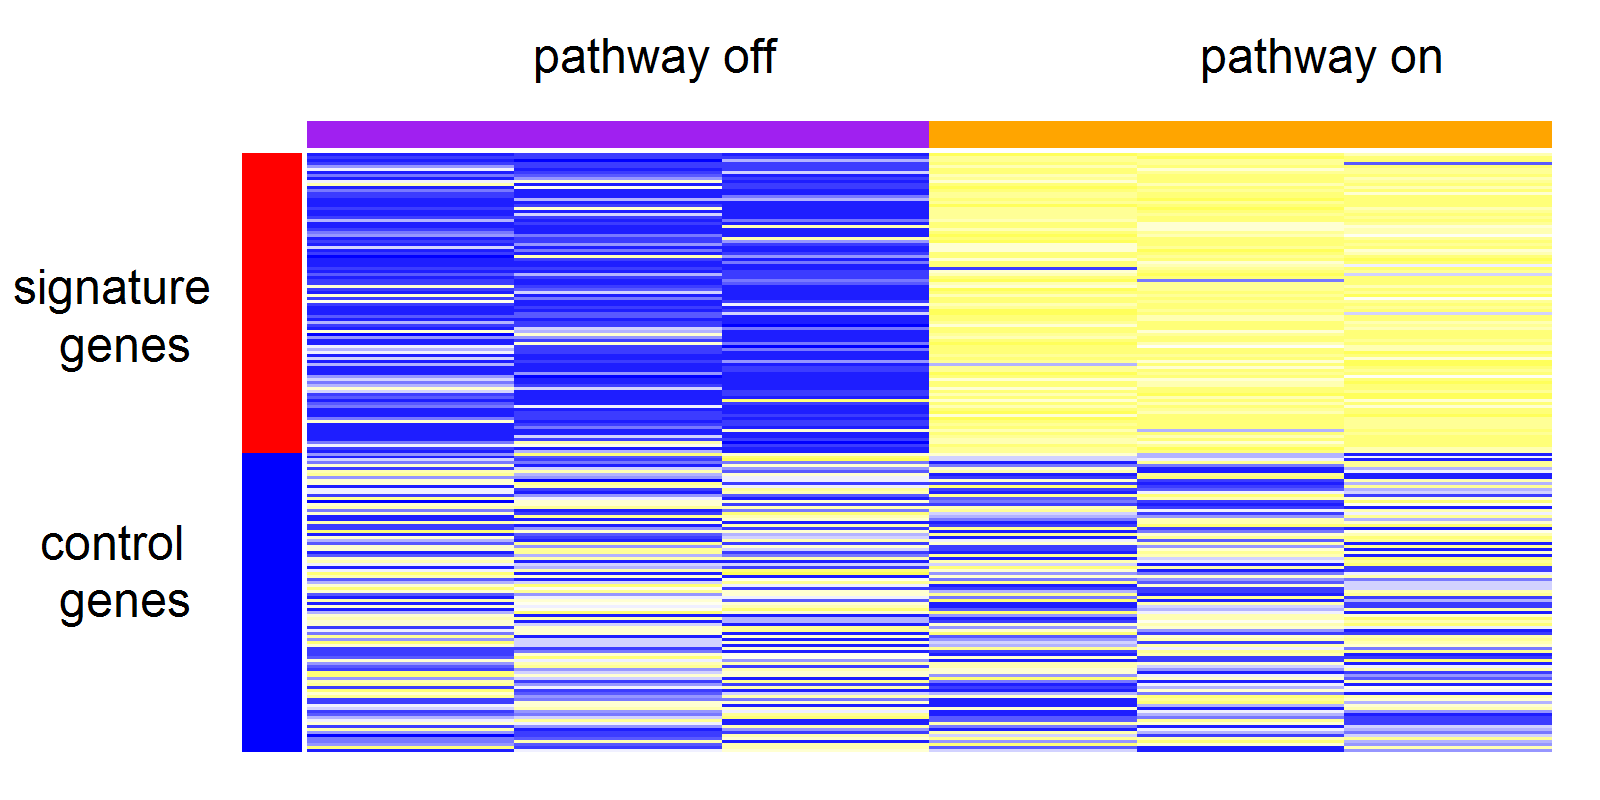
\includegraphics[width=0.45\textwidth]{batch1_combat_null.png}} 
    		\quad
    		\subfigure[Batch 2]{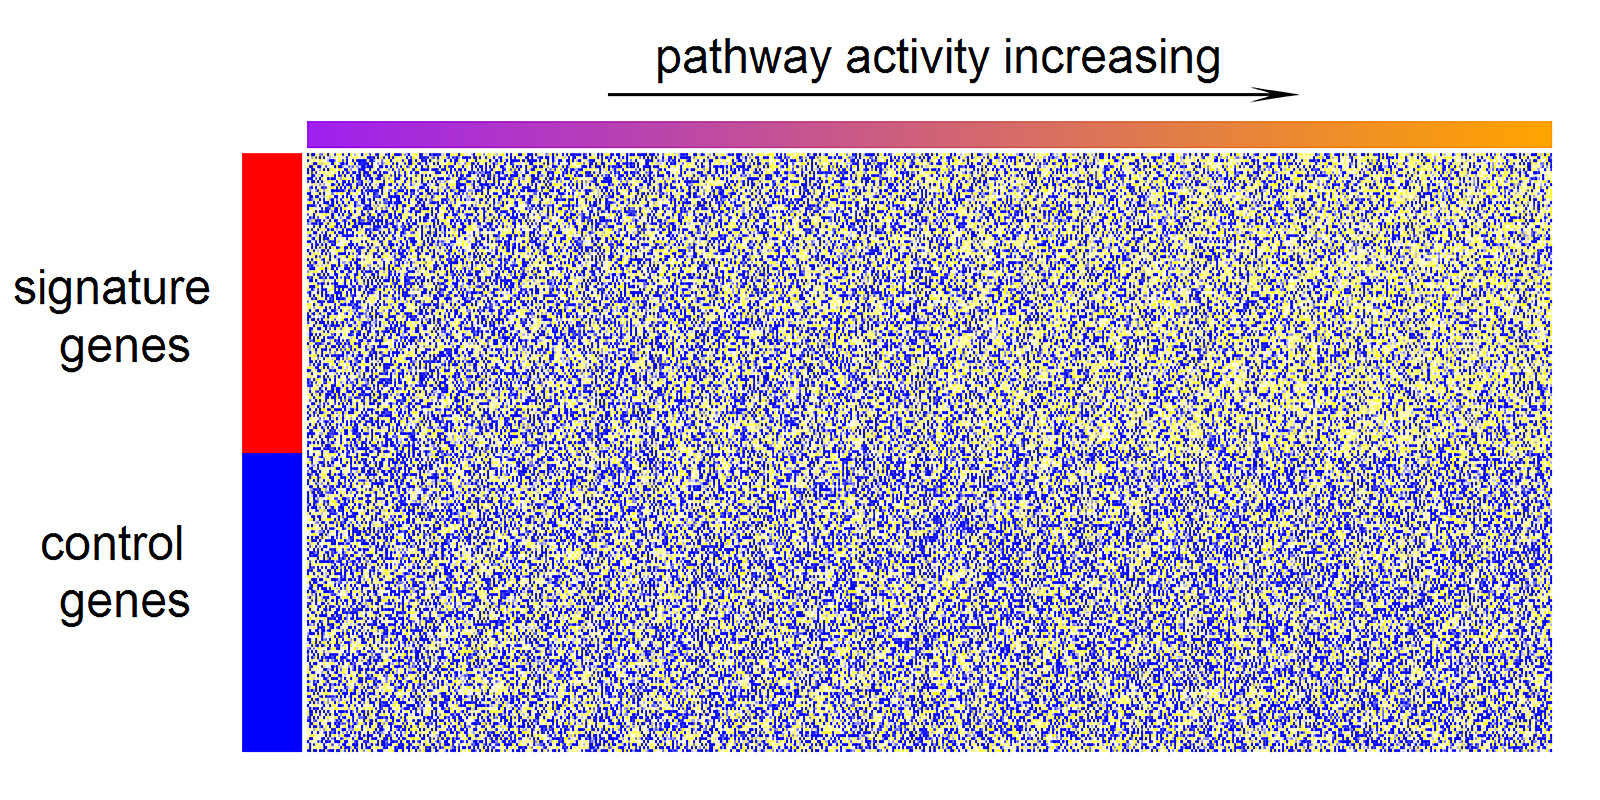
\includegraphics[width=0.45\textwidth]{batch2_combat_null.png}} 
   	 	}  \\
   	 	\renewcommand\thesubfigure{\textbf{B.}}
   	 	\subfigure[Reference-batch ComBat]{
   	 		%\setcounter{subfigure}{0}
   	 		\renewcommand\thesubfigure{}
    		\subfigure[Batch 1]{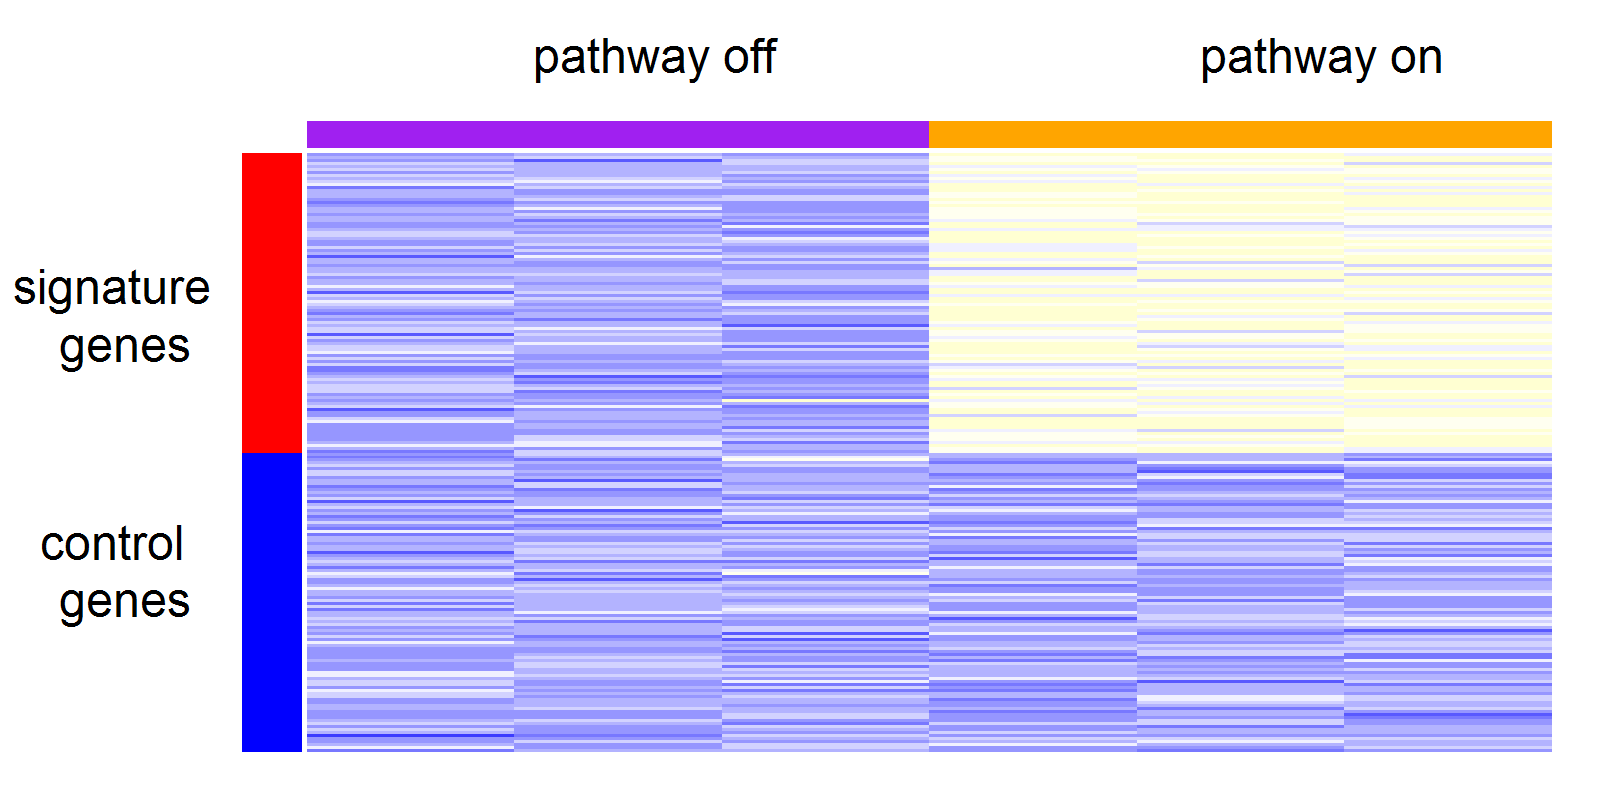
\includegraphics[width=0.45\textwidth]{batch1_refcombat_null.png}} 
    		\quad
    		\subfigure[Batch 2]{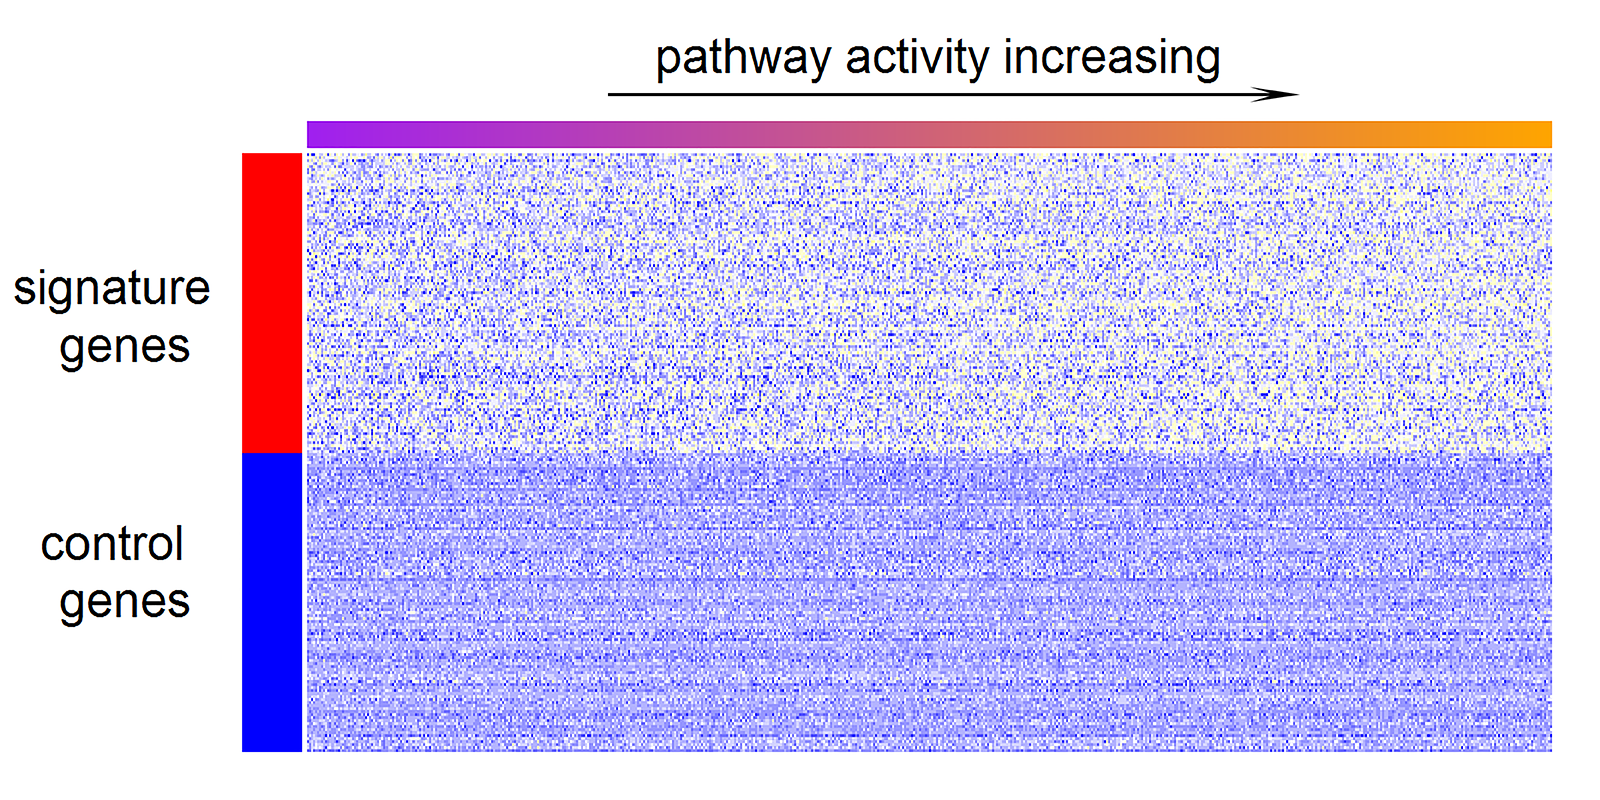
\includegraphics[width=0.45\textwidth]{batch2_refcombat_null.png}}
   	 	}
  	\end{center}
\end{figure}

\end{document}